% The entire content of this work (including the source code
% for TeX files and the generated PDF documents) by 
% Hongxiang Chen (nicknamed we.taper, or just Taper) is
% licensed under a 
% Creative Commons Attribution-NonCommercial-ShareAlike 4.0 
% International License (Link to the complete license text:
% http://creativecommons.org/licenses/by-nc-sa/4.0/).
\documentclass{article}

% My own physics package
% The following line load the package xparse with additional option to
% prevent the annoying warnings, which are caused by the package
% "physics" loaded in package "physicist-taper".
\usepackage[log-declarations=false]{xparse}
\usepackage{physicist-taper}


\makenomenclature % For an index of symbols.

% Show the keys for labels, replace options with "final" when done
% with editing.
\usepackage[draft,notref]{showkeys}

\title{Notes of Topological Transition in a Non-Hermitian Quantum Walk}
\date{\today}
\author{Taper}


\begin{document}


\maketitle
\abstract{
As suggested by the title.
}
\tableofcontents
\section{General}
\label{sec:General}

This paper discusses in general a model charaterised by the follwoing
picture
\begin{figure}[H]
    \centering
    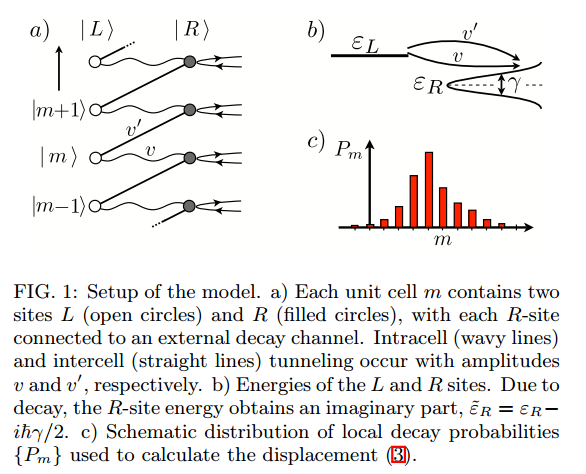
\includegraphics[width=0.8\linewidth]{pics/setup.PNG}
    \caption{Setup}
\end{figure}
The equation of motion is
\begin{align}
    \begin{aligned}
        \label{eq:eq-of-motion}
    i\hbar \dot{\psi}^L_m = \varepsilon_L\psi^L_m + v\psi^R_m
    +v'\psi^R_{m+1} \\
    i\hbar \dot{\psi}^R_m = \tilde{\varepsilon}_R\psi^R_m + v\psi^L_m
    +v'\psi^L_{m-1}
    \end{aligned}
\end{align}

where
\begin{equation}
    \tilde\varepsilon_R = \varepsilon_R - i\hbar \gamma/2
\end{equation}

\textbf{Important Note}: Through out the text we use $m$ as an
abbreviation of $R_m$. So $\psi_m$ means $\psi(R_m)$, $e^{ikm}$ means
$e^{ikR_m}$, and quite decivingly, $e^{ik}$~actually is $e^{ikR_1}$.

\subsection{I can get}
\label{sec:I-can-get}

\begin{equation}
    \ket{\psi} = \sum_m \ket{\psi_m^L} + \ket{\psi_m^R}
\end{equation}
\begin{equation}
    \frac{\partial }{\partial t}\braket{\psi|\psi}
    = -\sum_m \gamma \braket{\psi^R_m|\psi^R_m}
\end{equation}
(All leakage from "R" site!)
(draft page 1 to 2)

\colorbox{red}{Strange:}
\begin{equation}
    \sum_m P_m = 1
\end{equation} (draft page 3)
\subsection{Result}
\label{sec:Result}

\begin{myquote} \enquote{
we find that the average displacement
of the particle during the course of its decay, $\Delta m =\sum_m mP_m$, 
is exactly quantized as an integer (0 or 1 unit
cells), where $P_m$ is the probability distribution for decay from
different sites.

As in the case of
the quantum Hall conductance, this quantization results
from an underlying topological structure; in this case it
is the winding number of the relative phase between two
components of the Bloch wave function.

Using the topological origin of this phenomenon, we are able to show
that the quantization is insensitive to parameters and is
robust against certain types of noise and decoherence.

The topological transition, which is accompanied by the formation of
a non-decaying dark state, leads to a prediction of threshold-like
pumping of nuclear polarization, along with strong suppression of
current due to the divergence of dwell time at the threshold
} \end{myquote}

\begin{myquote} \enquote{
our motivation is to provide a simple
model of nuclear spin pumping in spin-blockaded double
quantum dots [9, 10, 11] in the presence of competing
effects of the hyperfine and spin-orbital interactions, as
in Ref.[11].
} \end{myquote}

\section{Calculation}
\label{sec:Calculation}


The system starts with the initial state:
\begin{equation}
    \psi^L_m = \delta_{m,0},\quad \psi^R_m = 0
\end{equation}

It evolves according to the following equation of motion
\ref{eq:eq-of-motion}:
\begin{align*}
    \begin{aligned}
    i\hbar \dot{\psi}^L_m = \varepsilon_L\psi^L_m + v\psi^R_m
    +v'\psi^R_{m+1} \\
    i\hbar \dot{\psi}^R_m = \tilde{\varepsilon}_R\psi^R_m + v\psi^L_m
    +v'\psi^L_{m-1}
    \end{aligned}
\end{align*}

The paper seeks to find the following:
\begin{align}
    \braket{\Delta m} &:= \sum_m m P_m \\
    P_m &:= \sum_0^\infty \gamma\abs{\psi^R_m(t)}^2 \dd t
    \label{eq:pm-def}
\end{align}
The result can be obtained both numerically and analytically. First,
the author provides an analytical solution.

\subsection{Analytical Solution}
\label{sec:Analytical-Solution}

\subsubsection{First observation}
\label{sec:First-observation}

The first thing the author points out is that:
\begin{equation}
    \frac{\partial }{\partial t}\abs{\psi}^2
    = \frac{\partial }{\partial t}  \braket{\psi|\psi} \neq 0
\end{equation}
This is caused by one fundamentabl rule of inner product:
\begin{equation}
    \frac{\partial }{\partial t}\braket{f|g} = 
    \braket{\frac{\partial f}{\partial t}|g} +
    \braket{g| \frac{\partial f}{\partial t}}
\end{equation}
The evolution of kets is determined by Schordinger's equation, the
evolution of bras is determined by conjugating the Schordinger's
equation. Thus, it is easy to see:
\begin{equation}
    \label{eq:pt-norm-1}
    i\hbar \frac{\partial }{\partial t}\abs{\psi}^2 =
    i\hbar \frac{\partial }{\partial t}\braket{\psi|\psi} =
    \bra{\psi} H-H^\dagger \ket{\psi}
\end{equation}
Applying the above rules here, we easily find (notice the only
non-hermitian term in the equation of motion \ref{eq:eq-of-motion} is
$\tilde\varepsilon_R = \varepsilon_R -i\hbar \gamma/2$, so
$H-H^\dagger$ is 
$\tilde\varepsilon_R-\tilde\varepsilon_R^*=-i\hbar\gamma$. This also
explains why author choose $\gamma/2$ in $\tilde\varepsilon_R$,
instead of $\gamma$. Thus we have
\begin{align}
    \label{eq:pt-norm-2}
    \frac{\partial }{\partial t}\braket{\psi^R_m|\psi^R_m} = 
    -\gamma \braket{\psi^R_m|\psi^R_m}
\end{align}
For the $L$ sites, the Hamiltonian is hermitian and thus
\begin{align}
    \frac{\partial }{\partial t}\braket{\psi^L_m|\psi^L_m} = 0
\end{align}

Counting them together, we let
\begin{equation}
    \ket{\psi} = \sum_m \ket{\psi^R_m} + \ket{\psi^L_m}
\end{equation}
and find
\begin{equation}
    \frac{\partial }{\partial t}\abs{\psi}^2 =
    \frac{\partial }{\partial t}\braket{\psi|\psi} =
    - \sum_m \gamma\braket{\psi^R_m|\psi^R_m}
\end{equation}

But he the author asserts
\begin{equation}
    \sum_m P_m = 1
\end{equation}
If we perceive that $P_m$ are probabilities, then the above equation
seems logical. But if I write down the formula (by eq \ref{eq:pm-def}):
\begin{equation}
    \sum_m P_m = \sum_m \int_0^\infty \gamma\braket{\psi^R_m|\psi^R_m}
    \overset{?}{=}1
\end{equation}
Then the result is not so obvious.\label{confusion:1}

\subsubsection{Pass to momentum space}
\label{sec:Pass-to-momentum-space}

The basic technique is fourier expansion
\begin{equation}
    \psi = \frac{1}{2\pi} \oint \dd{k} e^{ikm}\psi^R_m
\end{equation}
So the equation of motion \ref{eq:eq-of-motion} become:
\begin{align*}
    i\hbar \frac{\partial }{\partial t}\frac{1}{2\pi}
    \oint \dd{k} e^{ikm} \psi^L_k 
    =\frac{1}{2\pi} \oint \dd{k}  
    \left( \varepsilon_L e^{ikm}\psi^L_k
    + v e^{ikm}\psi^R_k + v' e^{ik(m+1)}\psi^R_k \right)
\end{align*}
similar to the other for $\psi^R_m$.  
The two equations can be simplified to (comparing the terms inside
integration):

\begin{align}
    \label{eq:eq-of-motion-in-k}
    \begin{aligned}
    i\hbar \dot{\psi}^L_k = \varepsilon_L\psi^L_k + v\psi^R_k
    +v' e^{ik} \psi^R_k \\
    i\hbar \dot{\psi}^R_k = \tilde{\varepsilon}_R\psi^R_k + v\psi^L_k
    +v'e^{-ik}\psi^L_{k}
    \end{aligned}
\end{align}

Or in matirx form:
\begin{equation}
    \label{eq:eq-of-motion-in-k-mat}
    i\hbar \frac{\partial }{\partial t}
        \begin{pmatrix}
            \psi^L_k \\ \psi^R_k
        \end{pmatrix}
        =
        \begin{pmatrix}
            \varepsilon_L & A_k \\
            A_k^* & \tilde\varepsilon_R
        \end{pmatrix}
        \begin{pmatrix}
            \psi^L_k \\ \psi^R_k
        \end{pmatrix}
\end{equation}
where $A_k:=v+v'e^{ik}$, and we have asumed $v,v'\in\R$. This is
Eq.(4) in the paper, and can be viewed as an Schordinger's equation in
the momentum space, with $H(k)$ the matrix on the right-hand-side.

By exactly the same technique described from Eq.~\ref{eq:pt-norm-1} to
Eq.~\ref{eq:pt-norm-2}, we can get:
\begin{align*}
    i\hbar\frac{\partial }{\partial t}\braket{\psi^L_k|\psi^L_k} &= 0
    \\
    i\hbar\frac{\partial }{\partial t}\braket{\psi^R_k|\psi^R_k} &= 
        -\gamma\braket{\psi^R_k|\psi^R_k}
\end{align*}

So (let $p_k(t):=\abs{\psi^L_k(t)}^2+\abs{\psi^R_k(t)}^2$):
\begin{equation}
    \frac{\partial }{\partial t}p_k = -\gamma\abs{\psi^R_k(t)}^2
    \label{eq:pt-pk}
\end{equation}

Notice
\begin{equation*}
    -\frac{i}{2\pi}\oint \dd{k} 
    \frac{\partial }{\partial k}(e^{ikm})\ket{\psi^R_k}
    =-i (im) \frac{1}{2\pi}\oint\dd{k} e^{ikm}\ket{\psi^R_k}
    =m\ket{\psi^R_m}
\end{equation*}

Then
\begin{align*}
    m\ket{\psi^R_m} &= -i \frac{1}{2\pi}\oint\dd{k}
    \frac{\partial }{\partial k}(e^{ikm})\ket{\psi^R_k}
    \\
    &=-i\frac{1}{2\pi}\left(
        \eval{e^{ikm}\ket{\psi^R_k}}_{\partial\textrm{BZ}}
        -\oint\dd{k} e^{ikm}\frac{\partial }{\partial k}\ket{\psi^R_k}
    \right)
    \\
    &= i\frac{1}{2\pi}\oint\dd{k}e^{ikm}\frac{\partial }{\partial k}
    \ket{\psi^R_k}
\end{align*}
Hence
\begin{align}
    \braket{\Delta m} &= \sum_m m\int_0^\infty
    \gamma\braket{\psi^R_m|\psi^R_m} 
    = \sum_m \int_0^\infty \gamma
    \bra{\psi^R_m} m\ket{\psi^R_m} \dd t
    \\
    &= \sum_m \int_0^\infty \gamma
    \left(\frac{1}{2\pi}\oint\dd{k} e^{-ikm}\bra{\psi^R_k}\right)
    i\frac{1}{2\pi}\oint\dd{k'}e^{ik'm}\frac{\partial }{\partial k}
        \ket{\psi^R_k} \\
    &= \sum_m \int_0^\infty \gamma
    \frac{i}{(2\pi)^2}\oint\dd{k}\dd{k'} e^{i(k'-k)m}
    \bra{\psi^R_k}\frac{\partial }{\partial k}\ket{\psi^R_k}
\end{align}
Noticing
\begin{equation}
    \sum_m e^{i(k'-k)m} = \delta(k'-k)\frac{(2\pi)^d}{v}
\end{equation}
where $v$ is the volumn of the primitive cell in real lattice and $d$
is the dimention of the real lattice.
So
\begin{align}
    \braket{\Delta m}
    &= \int_0^\infty \frac{i\gamma}{2\pi v}
    \oint\dd{k} \bra{\psi^R_k}
        \frac{\partial }{\partial k}\ket{\psi^R_k}
\end{align}
This same of Eq.(5) in the paper except a constant $v$.
\label{confusion:2}.

Next he sets $\ket{\psi^R_k}=u_k(t)e^{i\theta_k(t)}$, where $u$ is the
length and $\theta$ is the angle, of $\ket{\psi^R_k}$.

The author notes in [18] that the $u_k(t)>0$ for $t>0$, but this is
obvious from Eq.\ref{eq:pt-pk}, which is translated into
\begin{equation}
    \frac{\partial }{\partial t}(u_k)^2 = -\gamma (u_k)^2
\end{equation}
Thus $(u_k)^2$ is an exponential function, which is always positive
unless the initial condition is $0$.

Note
\begin{equation}
    \oint\dd{k} u_k\partial_k u_k 
    = \frac{1}{2}\oint\dd{k}\partial_k (u_k)^2 =
    \frac{1}{2}\eval{(u_k)^2}_{\textrm{\tiny two points of the same value}} = 0
\end{equation}
Then
\begin{figure}[H]
    \centering
    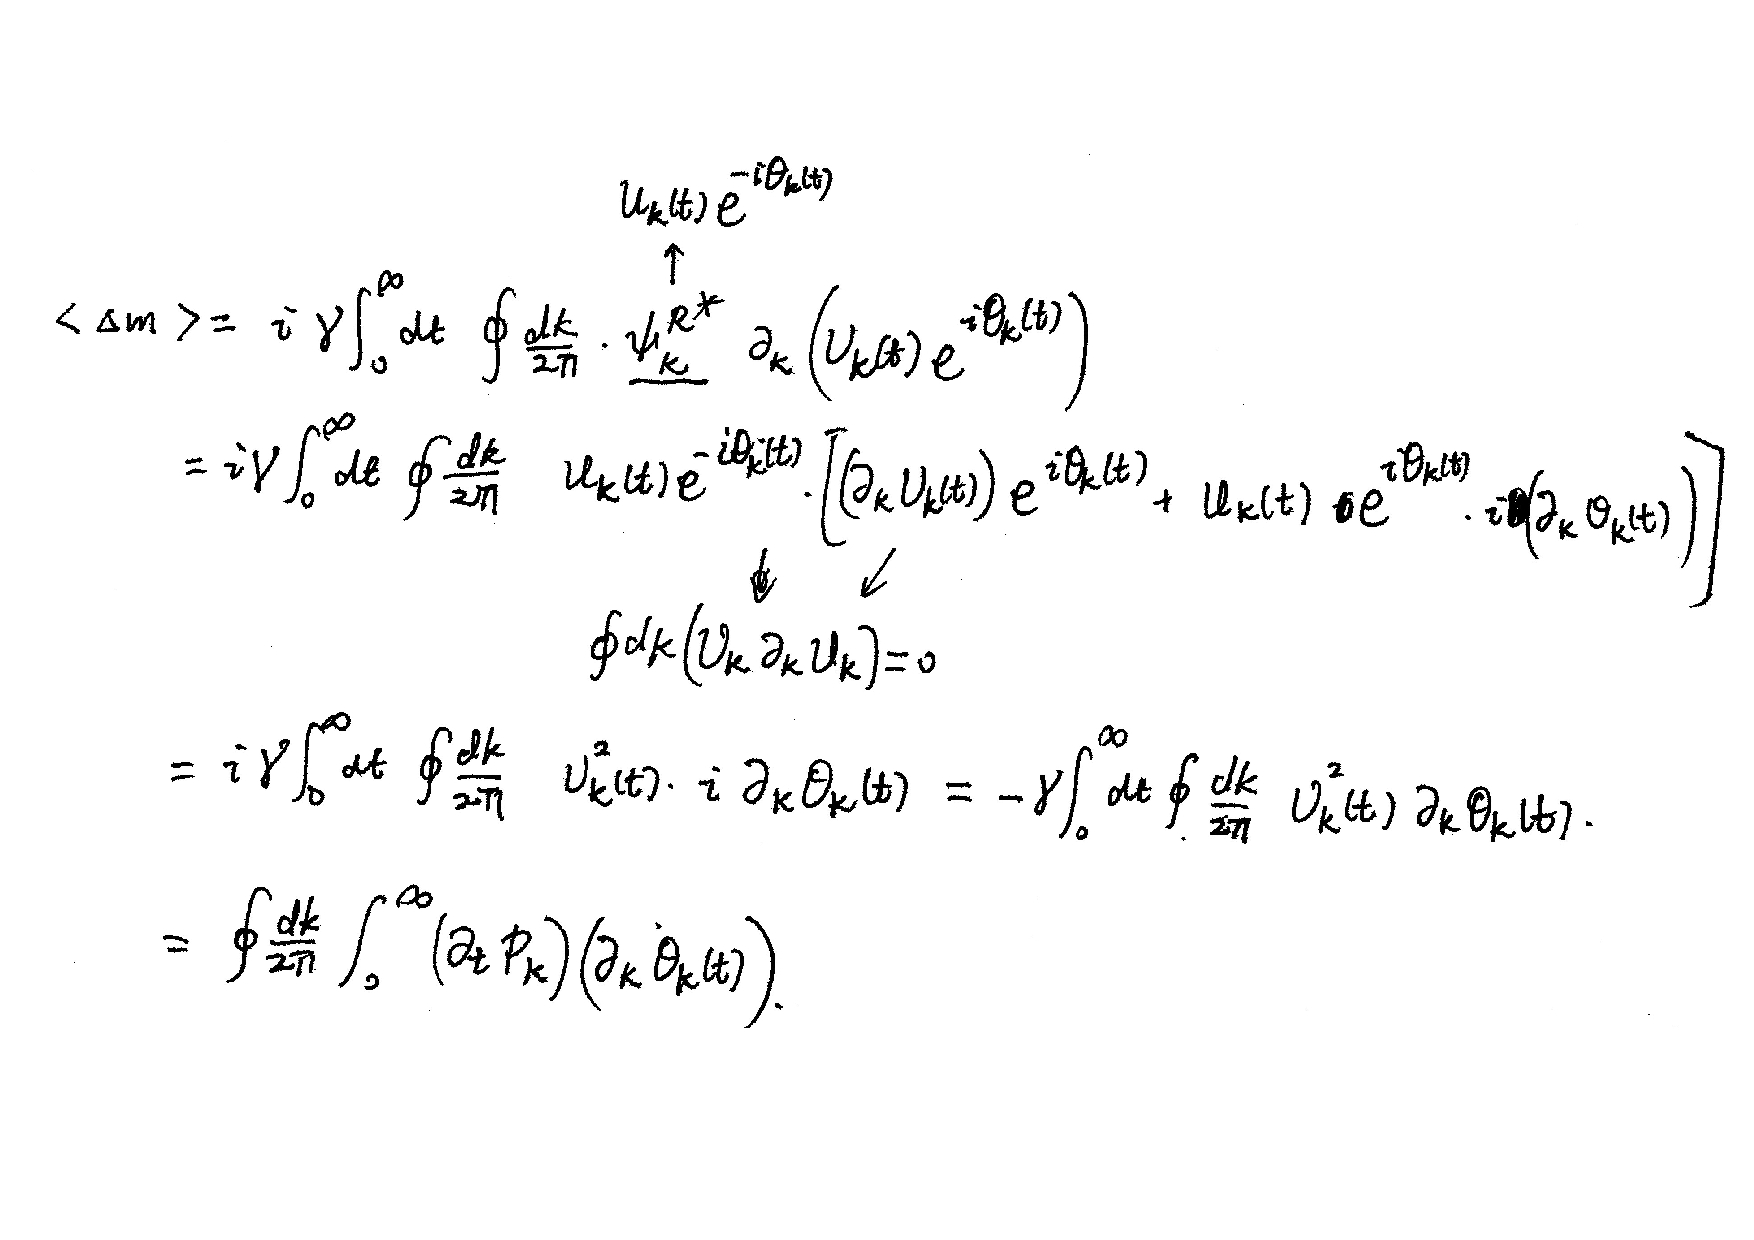
\includegraphics[width=0.8\linewidth]{pics/eq7.pdf}
\end{figure}
so
\begin{equation}
    \braket{\Delta m}=\oint\frac{\dd{k}}{2\pi}\int_0^\infty\dd{t}
    (\frac{\partial p_k}{\partial t})
    (\frac{\partial \theta_k(t)}{\partial k})
\end{equation}
This is Eq.7 in the paper, except that I have ignored the $\frac{1}{v}$
difference between my result and the paper's. Then it is straight
forward to obtain
\begin{equation}
    \braket{\Delta m} = \mathcal{I}_0 - \int_0^\infty\dd{t}
    \oint\frac{\dd{k}}{2\pi} p_k \partial_t (\partial_k \theta_k)
    \label{eq:m-I0-int}
\end{equation}
where
\begin{equation}
    \mathcal{I}_0 = \oint\frac{\dd{k}}{2\pi} \left(p_k
    \eval{\frac{\partial \theta_k}{\partial k}}_{t=0}^\infty\right)
\end{equation}
Now the second term in eq.\ref{eq:m-I0-int} can be turned into
(assuming $\theta_k(t)$ is smooth so that order of differentiation
does not matter).
\begin{equation}
    - \int_0^\infty\dd{t}
    \oint\frac{\dd{k}}{2\pi} p_k \partial_t (\partial_k \theta_k)
    =
    \int_0^\infty\dd{t}
    \oint\frac{\dd{k}}{2\pi} 
    \frac{\partial p_k}{\partial k}
    \frac{\partial \theta_k}{\partial t}
    \label{eq:to-be-0}
\end{equation}
This is eq.(9) in the paper.

\subsubsection{Arguing that the Integration \ref{eq:to-be-0} is zero}
\label{sec:Argument-1}

Now the author tries to argue that $p_k$ and $\partial_t\theta_k$ are
even functions of $k$, so that the integration \ref{eq:to-be-0} is $0$.
I cannot follow his argument
\label{confusion:3}. But I find another model, which can found on
\href{https://en.wikipedia.org/wiki/Rabi_cycle}{Wikipedia - Rabi
Cycle}. The Rabi Cycle model can be applied only when $\gamma=0$, i.e.
there is no dissipation. But since the formulae above are continues,
if the integration $p_k$ and $\partial_t\theta_k$ are even, then they
should be even when $\gamma=0$, unless some very strange singular
behavior exist.


\paragraph{$\gamma=0$ case using Two-level system model}$ $


Suppose we have a Hermitian Hamiltonian (let
$\{E_0,W_1,W_2,\Delta\}\subset\R$):
\begin{equation}
    H = E_0\id + W_1\sigma_1+W_2\sigma_2+\Delta\sigma_3 
    = \begin{pmatrix}
        E_0 + \Delta & W_1-iW_2 \\
        W_1+iW_2 & E_0 - \Delta
    \end{pmatrix}
\end{equation}

Supose the system starts at $\ket{\psi(0)}= \begin{pmatrix}
    1\\0
\end{pmatrix}$, then its time evolution will be (Set $\hbar=1$.
Calculation is done in the Wikipedia page, and is checked myself.):
\begin{equation}
    \label{eq:time-evolve-rabi}
    \ket{\psi(t)} = \cos(\theta/2)e^{-iE_+ t}\ket{E_+} - \sin(\theta/2)
    e^{-i\phi}e^{-iE_- t}\ket{E_-}
\end{equation}
where $\ket{E_+}=e^{i\phi/2} \begin{pmatrix}
    \cos(\theta/2) \\ e^{-i\phi}\sin{\theta/2}
\end{pmatrix}$ and $\ket{E_-}= \begin{pmatrix}
    -e^{i\phi}\sin(\theta/2) \\ \cos(\theta/2)
\end{pmatrix}$ are orthonormal eigenkets, and
\begin{align}
\begin{aligned}
    &W:= W_1+iW_2,\quad
    E_{\pm} = E_0\pm \sqrt{\Delta^2+\abs{W}^2}\\
    &\sin(\theta):= \frac{|W|}{\sqrt{\Delta^2+\abs{W}^2}},\,
    \cos(\theta):= \frac{\Delta}{\sqrt{\Delta^2+\abs{W}^2}},\,
\end{aligned}
\end{align}
$\phi$ is such that $W=\abs{W}e^{-i\phi}$.

Here for this paper. Let us suppose for the moment $\gamma=0$, then we
see that $W=A_k^*$, so $W_1 = v+v'\cos{k}$, $W_2=-v'\sin{k}$. 
Also $E_0$ and $\Delta$ are linear combination of
$\varepsilon_R$ and $\varepsilon_L$:
\begin{equation}
    E_0 =\frac{\varepsilon_R+\varepsilon_L}{2},\quad
    \Delta =\frac{\varepsilon_R-\varepsilon_L}{2}
\end{equation}
The system still starts with
$\ket{\psi(0)}$ (since $\psi^L_k(0)=1,\,\psi^R_k(0)=0$). The time
evolved state still follows eq.\ref{eq:time-evolve-rabi}, where the
dependence on $k$ lies in $\sin(\theta),\cos(\theta),$ and $\phi$.
Then by definition, $p_k=\abs{\ket{\psi(t)}}^2$, $u_k(t)$ is the second
component of $\ket{\psi(t)}$.

I was doubtful of the fact that $p_k$ is even in $k$, so I did a
numerical check (see file
"{OneD\_quantum\_walk\_test\_even\_functions\_pk\_uk.m}"), and
unfortunately my guess seems to be wrong. I have given arbitrary
numbers to time $t$, $v$, $v'$, energies $\varepsilon_R$ and
$\varepsilon_L$, and the resulted $p_k$ is always even in $k$, the
resulted $u_k$ is always constantly $0$ in both time variable $t$ and $k$.

This motivates me to calculate it analytically. The results is
contained in files \\
"\texttt{Elementary Calculation of Time Evolution in Two-level model.nb}"

and\\
"\texttt{Elementary Calculation to get pk and uk from Two-Level
model.nb}".

(their pdf version files are also included) 

The result is that I can understand $p_k$ is even in $k$, but I cannot
see why $\partial_t u_k$ because its calculation involves getting the
angle of a complex number, which has not good analytical expressions.

\section{Anchor}
\label{sec:Anchor}

\begin{thebibliography}{1}
    \bibitem{1dwalk} Topological Transition in a Non-Hermitian Quantum
    Walk,
    \href{https://arxiv.org/ct?url=http%3A%2F%2Fdx.doi.org%2F10%252E1103%2FPhysRevLett%252E102%252E065703&v=f6968ad6}{arXiv}
\end{thebibliography}
\printnomenclature
\section{License}
The entire content of this work (including the source code
for TeX files and the generated PDF documents) by 
Hongxiang Chen (nicknamed we.taper, or just Taper) is
licensed under a 
\href{http://creativecommons.org/licenses/by-nc-sa/4.0/}{Creative 
Commons Attribution-NonCommercial-ShareAlike 4.0 International 
License}. Permissions beyond the scope of this 
license may be available at \url{mailto:we.taper[at]gmail[dot]com}.
\end{document}
